\documentclass[final]{fhnwreport}       %[mode] = draft or final
                                        %{class} = fhnwreport, article, 
                                        %          report, book, beamer, standalone
%%---Main Packages-----------------------------------------------------------------------
\usepackage[english, ngerman]{babel}	%Mul­tilin­gual sup­port for LaTeX
\usepackage[T1]{fontenc}				%Stan­dard pack­age for se­lect­ing font en­cod­ings
\usepackage[utf8]{inputenc}				%Ac­cept dif­fer­ent in­put en­cod­ings
\usepackage{lmodern}                    %The newer Font-Set
\usepackage{textcomp}					%LaTeX sup­port for the Text Com­pan­ion fonts
\usepackage{caption}					%Customising captions in floating environments
\usepackage{graphicx} 					%En­hanced sup­port for graph­ics
\usepackage{float}						%Im­proved in­ter­face for float­ing ob­jects
\usepackage{ifdraft}                    %Let you check if the doc is in draft mode
\usepackage{enumitem}


%%---Useful Packages---------------------------------------------------------------------
\usepackage{colortbl}	
\usepackage{color}						%Colour control for LaTeX documents
\usepackage[pdftex,dvipsnames,tabl]{xcolor}  %Driver-in­de­pen­dent color ex­ten­sions for LaTeX
\usepackage{csquotes}                   %Simpler quoting with \enquote{}
\usepackage{siunitx} 					%A com­pre­hen­sive (SI) units pack­age
%\usepackage{listings}					%Type­set source code list­ings us­ing LaTeX
\usepackage[bottom]{footmisc}			%A range of foot­note op­tions
\usepackage{footnote}					%Im­prove on LaTeX's foot­note han­dling
\usepackage{verbatim}					%Reim­ple­men­ta­tion of and ex­ten­sions to LaTeX ver­ba­tim
\usepackage[textsize=footnotesize]{todonotes} %Mark­ing things to do in a LaTeX doc­u­ment
\usepackage{titling}					%Control over the typesetting of the \maketitle command
\usepackage[euler]{textgreek}		%Allows to write greek letters without entering math-mode (\textOmega)

%%---Tikz Packages-----------------------------------------------------------------------
\usepackage{standalone}
\usepackage{tikz}
\usepackage{circuitikz}
\usetikzlibrary{arrows}
\usetikzlibrary{calc}
\usetikzlibrary{intersections}

%%---Math Packages-----------------------------------------------------------------------
\usepackage{amsmath}					%AMS math­e­mat­i­cal fa­cil­i­ties for LaTeX
\usepackage{amssymb}					%Type­set­ting symbols (AMS style)

%\usepackage{amstext}
%\usepackage{amsfonts}
%\usepackage{breqn}
%\usepackage{array}						%Ex­tend­ing the ar­ray and tab­u­lar en­vi­ron­ments
%\usepackage{amsthm}					%Type­set­ting the­o­rems (AMS style)

%%---Table Packages----------------------------------------------------------------------
\usepackage{tabularx}					%Tab­u­lars with ad­justable-width columns
%\usepackage{longtable}
%\usepackage{multirow}					%Create tab­u­lar cells span­ning mul­ti­ple rows
\usepackage{multicol}					%In­ter­mix sin­gle and mul­ti­ple columns



%%---PDF / Figure Packages---------------------------------------------------------------
\usepackage{pdfpages}					%In­clude PDF doc­u­ments in LaTeX
%\usepackage{pdflscape}					%Make land­scape pages dis­play as land­scape
%\usepackage{subfig}					    %Fig­ures di­vided into sub­fig­ures

%%---Other Packages----------------------------------------------------------------------
%\usepackage{xargs}                     %De­fine com­mands with many op­tional ar­gu­ments


%%---Bibliography------------------------------------------------------------------------
\usepackage[style=ieee,urldate=comp,backend=biber]{biblatex}
\addbibresource{literature/bibliography.bib}

%%---Main Settings-----------------------------------------------------------------------
\graphicspath{{./graphics/}}			%Defines the graphicspath
\geometry{twoside=false}				    %twoside=false disables the "bookstyle"
\setlength{\marginparwidth}{2cm}
\overfullrule=5em						%Creates a black rule if text goes over the margins => debugging




%%---User Definitions--------------------------------------------------------------------
%%Tabel-Definitions: (requires \usepackage{tabularx})
\newcolumntype{L}[1]{>{\raggedright\arraybackslash}p{#1}}    %column-width and alignment
\newcolumntype{C}[1]{>{\centering\arraybackslash}p{#1}}
\newcolumntype{R}[1]{>{\raggedleft\arraybackslash}p{#1}}
\usepackage{subcaption}


%%---Optional Package Settings-----------------------------------------------------------
%Listings-Settings: (requires \usepackage{listings}) => Example with Matlab Code
%\lstset{language=Matlab,%
%    basicstyle=\footnotesize\ttfamily,
%    breaklines=false,%
%    morekeywords={switch, case, otherwise},
 %   keywordstyle=\color{Blue},%
 %  tabsize=2,
    %morekeywords=[2]{1}, keywordstyle=[2]{\color{black}},
%    identifierstyle=\color{Black},%
%    stringstyle=\color{Purple},
%    commentstyle=\color{Green},%
%    showstringspaces=false,%without this there will be a symbol in the places where there is a space
%    numbers=left,%
%    numberstyle={\tiny \color{black}},% size of the numbers
%    numbersep=9pt, % this defines how far the numbers are from the text
    %emph=[1]{word1, word2,...},emphstyle=[1]\color{red}
%}							

%Hurenkinder und Schusterjungen verhindern (kein Scherz, Google es)
\clubpenalty10000
\widowpenalty10000
\displaywidowpenalty=10000	



%Titel mit Mathematik immer fett drucken
\usepackage{sectsty}
\allsectionsfont{\boldmath}



			                %loads all packages, definitions and settings											
\title{Fachliches Pflichtenheft}  		        %Project Title
\author{Team 1}      				    %Document Type => Technical Report, ...
\date{\today}          				   %Place and Date

\begin{document}

%%---TITLEPAGE---------------------------------------------------------------------------------
\thispagestyle{empty}
%	\ohead{\includegraphics[scale=0.5]{Bilder/Logo_FHNW.jpg}}
	\begin{figure}
		 \vspace*{-\topskip}\vspace*{-\headsep}
		
\includegraphics[scale=1]{graphics/fhnw_ht_logo_de.pdf}
	\end{figure}
	\begin{center}
		\vspace*{2cm}
		{\huge{\textbf{\thetitle}}}\\
		\vspace*{0.5cm}
		
		{\scshape\Large Projekt 4 - \theauthor \\} \Large{\today}
		\vfill
		\begin{normalsize}
			{\begin{tabbing}
					\textbf{Auftraggeber:} \hspace{5cm}\= Prof. Hans Gysin\\
					
					\\[0.8cm]
					\textbf{Fachcoach:} 
					\>Prof. Dr. Pascal Schleuniger\\
					\>Matthias Meier\\
					\>Albert Zihlmann\\
					\>Dr. Anita Gertiser\\
					\>Pascal Buchschacher\\
					\>Marie-Thérèse Rudolf von Rohr\\
					
					\\[0.4cm]
					\textbf{Projektleiter:} \>Fabian von Büren\\
					\\[0.4cm]
					
					\textbf{Team:} \>Christoph Kuhn \\ \>Dennis Aeschbacher \\ \>Raffael Anklin \\ \>Raphael Nikles \\ \>Robin Aebi
					\\[0.8cm]
					\textbf{Studiengang:} \>Elektro- und Informationstechnik
					\\[0.8cm]	\textbf{Semester:} \>Frühlingssemester 2019
			\end{tabbing}}
		\end{normalsize}
		\vfill
	\end{center}
\clearpage


%%---TABLE OF CONTENTS-------------------------------------------------------------------
\pagenumbering{Roman}		
\selectlanguage{ngerman}				%ngerman or english
\tableofcontents
\clearpage

%%---TEXT--------------------------------------------------------------------------------
\pagenumbering{arabic}
	\clearpage
\section{Übersicht}\label{sec:Uebersicht}

In diesem Kapitel soll eine Übersicht über den Inhalt des Projekt 4 des Studiengangs Elektro- und Informationstechnik gegeben werden. Dabei soll auch aufgezeigt werden, welche Ziele erreicht werden sollen und welche Lieferobjekte erstellt werden müssen. 

 









	
\subsection{Ausgangslage}\label{subsec:Ausgangslage}

Vor nicht allzulanger Zeit war der Bau von Prototypen oder Modellen eine Herausforderung, da es aufwändig war komplexere Formen zu modellieren und aufzubauen. 1981 wurde erstmals ein 3D-Drucker entwickelt, welcher es ermöglichte mittels Stereolithographie\footnote{\textbf{Stereolithografie} ist das älteste additive Fertigungsverfahren, bei dem ein Werkstück durch frei im Raum aufgetragene Rasterpunkte schichtenweise aufgebaut wird. Die Fertigung eines Werkstückes erfolgt vollautomatisch aus am Computer erstellten CAD-Daten.} eine komplexe Figur zu modellieren. Dies war der Anfang eines neuen technischen Zeitalters. Das Problem war jedoch, dass 3D-Drucker zu Beginn enorm teuer waren. Heutzutage sind diverse 3D-Drucker auf dem Markt, welche mittels unterschiedlicher Methoden dreidimensionale Objeke erschaffen. Diese sind mittlerweile auch für jedermann erschwinglich. Im Projekt 4 soll die Elektronik für einen 3D-Drucker entwickelt werden, welcher mittels \textit{Fused Deposition Modeling} Werkstücke kreiert. Dabei wird ein Kunststoffstrang geschmolzen und durch eine feine Düse gepresst. Der Extruder (Druckkopf) baut dann mit dem austretenden Kunststofffaden Schicht um Schicht ein dreidimensionales Objekt auf \cite{3D_Druckverfahren}\cite{Fused_Deposition_Modeling}.









	\clearpage
\subsection{Projektziele}\label{subsec:Projektziele}
In Tabelle \ref{tab:PlfichtundWunschziele} sind die Pflicht- und Wunschziele für dieses Projekt festgehalten. Diese sind an das Lastenheft des Auftraggebers angelehnt (siehe Anhang \ref{app:Lastenheft}).

\begin{table}[H]
\begin{tabular}{ | C{0.9cm} | p{9cm} | | p{4.5cm} |}
	\hline
	\multicolumn{3}{|l|}{\textbf{Pflichtziele}}\\ \hline
\textbf{Nr.}& \textbf{Ziel}& \textbf{Messung der Zielerreichung}\\ \hline

P1& Unabhängige Ansteuerung aller vier Schrittmotoren (x-, y-, z-Achse und Zuführung Filament), ohne das Schritte verloren gehen.&		Testfahrt über Zeit mit Kontrolle der Schritte\\ \hline
    
P2& Nullpositions-Erkennung der x-, y- und z-Achse.&		Positionserkennung mit mindestens $\pm 1mm$ Genauigkeit\\ \hline
    
P3& Regelung der Heizleistung von Extruder und Heizbett.&		Erreichen der Solltemperatur auf $\pm5^\circ C$\\ \hline
    
P4& Temperaturmessung für Extruder und Heizbett.&		Messgenauigkeit auf $\pm5^\circ C$\\ \hline
    
P5& Ansteuerung eines Ventilators (Kühlung der bereits gedruckten Strukturen).& Strukturen werden entsprechend gekühlt\\ \hline
    	
P6& Laden von GCode via SD-Karte und WLAN.&		Datei befindet sich auf SD-Karte\\ \hline
    
P7& Bedienelemente um alle wichtigen Funktionen des 3D-Druckers zu steuern (Taster, LEDs, Display, etc.)&	Interaktion mit Drucker möglich.\\ \hline

P8& 3D-Drucker soll funktionsfähig sein.&		Testdruck erfolgreich\\ \hline

P9& Möglichkeit zur manuellen Ansteuerung (alle Achsen und Sensoren).&	Die gewünschte Aktionen werden korrekt ausgeführt\\ \hline

    	 \hline \hline   
 \multicolumn{3}{|l|}{\textbf{Wunschziele}}\\ \hline 	
    
    
W1& Detektion wenn kein Filament mehr vorhanden ist (optisch oder mechanisch).&		System setzt entsprechende Meldung ab\\ \hline

W2& Webseite mit Benutzeroberfläche um Druckaufträge zu verwalten zu verfolgen und abzurufen.&		Bedienung über Webseite möglich\\ \hline

W3& Möglichst geringer Eigenverbrauch im Ruhezustand.&		Eigenverbrauch liegt unterhalb der Standard Lösung\\ \hline

W4& Luftkanal für Ventilator herstellen (mechanische Änderung).&		Verbesserung der Kühlung\\ \hline

W5& Verwenden einer Glasplatte auf dem Heizbett für bessere Druckqualität (mechanische Änderung).&		Erreicht / nicht erreicht\\ \hline

W6& Verbesserung des Abrollvorgangs des Filaments (mechanische Änderung).&		Erreicht / nicht erreicht\\ \hline

W7& Kugellager durch Gleitlager ersetzen welche weniger verschleissen (mechanische Änderung).&		Erreicht / nicht erreicht\\ \hline

W8& Autoleveling der z-Achse.&		Erreicht / nicht erreicht\\ \hline

W9& Encoder anstatt Taster als Bedienelemente.&		Erreicht / nicht erreicht\\ \hline

\end{tabular}\\
\caption{Pflicht- und Wunschziele}
\label{tab:PlfichtundWunschziele}
\end{table}




















	\clearpage
\subsection{Lieferobjekte}\label{subsec:Lieferobjekte}
Zusätzlich zu den Projektzielen, folgen in diesem Kapitel die Lieferobjekte und wichtige Meilensteine mit dem jeweiligen Datum. In der Tabelle \ref{tbl:Lieferobjekte} sind diese detailliert aufgelistet.  


\begin{table}[H]
     \centering
\begin{tabular}{|c|c|l|}\hline
   \textbf{Nr.} & \textbf{Datum} & \textbf{Lieferobjekt} \\ \hline
   1 & 17.03.2019 & Abgabe Fachliches Pflichtenheft, erste Version \\ \hline 
   2 & 31.03.2019 & Abgabe Fachliches Pflichtenheft, definitive Version \\ \hline
   3 & 05.05.2019 & Abgabe Disposition und Einleitung Fachbericht \\ \hline
   4 & 07.05.2019 & G-Code drahtlos übermitteln \\ \hline   
   5 & 19.05.2019 & Abschluss Realisierung \\ \hline   
   6 & 02.06.2019 & Abschluss Validierung \\ \hline   
   7 & 11.06.2019 & Abgabe Fachbericht \\ \hline
   8 & 11.06.2019 & Abgabe Fact sheet \\ \hline
   9 & 11.06.2019 & Abgabe Produkt und dazugehörige Software \\ \hline   
   
 \end{tabular}
     \caption{Lieferobjekte und wichtige Meilensteine}
     \label{tbl:Lieferobjekte}
\end{table}










\pagebreak

\clearpage
\section{Lösungskonzept}\label{sec:Loesungskonzept}
In Abbildung \ref{img:Grobkonzept} ist das Blockschaltbild ersichtlich, welches alle Teilsysteme und Einheiten darstellt. Es ist modular gegliedert und bietet eine Übersicht der Schnittstellen zwischen den einzelnen Modulen. 

Das Lösungskonzept selbst gliedert sich in drei physikalisch getrennte Einheiten. Das \textit{Machine Controll System} (MCS), das \textit{Human Maschine System} (HMS) und den Drucker selbst, einen \textit{Ender 3} der Firma \textit{Creality3D}. 

Das MCS bildet den Hauptbestandteil des Lösungskonzepts. Es beinhaltet die Druckersteuerung und die Kommunikationsschnittstellen. Um diese zwei Aufgaben zu separieren befinden sich zwei Mikroprozessoren in dieser Einheit. Zusätzlich werden die Aktoren und Sensoren des 3D-Druckers  angesteuert und eingelesen. Eine Statusanzeige zur Visualisierung des Zustandes ist ebenfalls angedacht.

Das HMS bildet die Benutzerschnittstelle über ein internetfähiges Gerät. Es kommuniziert mittels WLAN mit dem MCS. Über dieses Gerät können Druckaufträge verwaltet und überwacht werden. Auf dem 3D-Drucker befinden sich alle Aktoren und Sensoren. Sie werden über Kabelverbindungen an das MCS angebunden.



\begin{figure}
	\centering
	\includegraphics[scale=0.58,angle=90]{19FS-pro4E-Team1_Grobkonzept_25022019_ohne_Rahmen.png}
	\caption{Blockschaltbild des Lösungskonzepts}
	\label{img:Grobkonzept}
\end{figure} 









\pagebreak

\clearpage
\section{Hardware / Machine Controlling System}\label{sec:Hardware}
Das \textit{Machine Controlling System} dient der Steuerung des 3D-Druckers sowie der Regelung einzelner Komponenten. Es setzt sich aus mehreren funktional verschiedenen Einheiten zusammen, welche in diesem Kapitel beschrieben werden.


\subsection{Motor Control Unit (MCU)}\label{subsec:MCU}
Die \textit{Motor Control Unit} ist für die Ansteuerung der Schrittmotoren zuständig. Es sollen vier Schrittmotoren angesteuert werden. Dabei handelt es sich um den Extrudermotor, welcher das Filament fördert und die drei Achsenmotoren für die x-, y- und z-Bewegungen. Die Ansteuerung soll mittels Motorentreiber realisiert werden. Der Mikrocontroller soll mit der Firmware \textit{Marlin} gemäss Kapitel \ref{subsec:PCU} arbeiten. Dabei stehen jedem Schrittmotor drei Digitalpins vom Mikrocontroller zur Verfügung. Dabei handelt es sich um einen Enable Pin (\textit{EN}), welcher den Treiber aktiviert, einem Signal (\textit{DIR}) für die Drehrichtung des Schrittmotors und einem Schrittgeber (\textit{STEP}), welcher jeweils mittels positiver Flanke den jeweiligen Schrittmotor um einen Schritt weiter dreht. 

Die Schrittmotoren können mit maximal 2.5A betrieben werden. Bei diesem Strom wird das maximale Drehmoment der Motoren erreicht. Im Betrieb soll das volle Drehmoment jedoch nicht erreicht werden, da die Motoren möglichst unbehindert arbeiten sollten. Die Treiber sollen daher auf einen maximalen Strom von $\sim$ 2A ausgelegt werden.

Die Schrittauflösung der Motoren beträgt $1.8^\circ$ pro Schritt. Dies ergibt eine Auflösung von 200 Schritten pro Umdrehung. Bei dem vormontierten Ritzel des \textit{Ender 3} 3D-Druckers ($\sim$ 13.9mm Durchmesser) ergibt dies einen Weg von 0.218mm pro Schritt in x- und y-Richtung. Da eine höhere Auflösung angestrebt wird, sollen die Motorentreiber microstepping\footnote{\textbf{Microstepping} treibt einen Schrittmotor mit weniger als einem Vollschritt pro Bewegung an. Unter normalen Betriebsbedingungen arbeitet ein Schrittmotor, indem er jeweils einen Vollschritt weiterdreht pro positive Flanke am STEP-Eingang. Microstepping ermöglicht es einem Motor, weitaus feinere Schritte zu machen. Dies geschieht, indem die Steuerung nicht den vollen Stromimpuls an den Schrittmotor sendet.} unterstützen von mindestens 16 Teilschritten pro Schritt ($\frac{1}{16}$). Somit kann eine Auflösung von mindestens 3200 Schritten pro Umdrehung erreicht werden. Dies ergibt wiederum einen Weg von $0.0136$mm pro Schritt. Dies ist jedoch nur eine Überschlagsrechnung. Eine genaue Kalibration kann, nach einem Testdruck, in der Software vorgenommen werden. 

Aus den erwähnten Gründen wurde ein Treiber von \textit{TMC} ausgewählt. Es handelt sich dabei um den \textit{TMC2130} \textit{SilentStepStick} Treiber. 

\subsection{Debugging Interface Unit (DIU)}\label{subsec:DIU}
Die \textit{Debugging Interface Unit} ist dazu da, das Debuggen während dem Entwicklungsprozess der Firmware zu vereinfachen. Via UART/USB-Bridge können Messwerte, Statewerte der aktuell verwendeten Zustandsmaschinen, etc. auf dem Computer ausgegeben werden. Aus Kostengründen würden die verwendeten Bauteile in einer Serienproduktion nicht bestückt werden und stellen daher eine Bestückungsvariante dar.

\subsection{Printer Controlling Unit (PCU)}\label{subsec:PCU}
Die \textit{Printer Controlling Unit} beinhaltet die nötige Schaltungsteile um den 3D-Drucker zu steuern bzw. zu regeln. Namentlich den zentralen Mikrocontroller und diverse Bussysteme welche nötig sind um die verwendete Peripherie anzusteuern. Als Grundlage für die Firmware des Mikrocontrollers wird die Firmware \textit{Marlin} verwendet \cite{marlin_webseite} welche unter \textit{GNU General Public License Version 3} frei verfügbar ist \cite{marlin_gnu_lizenz}. Aus Kompatibilitätsgründen zu den erforderlichen Pins der Firmware \textit{Marlin} wird als Mikrocontroller ein \textit{ATmega2560} \cite{ATmega2560_spezifiaktion} der Firma \textit{Microchip Technology} verwendet.

\subsection{Storage Disk Unit (SDU)}\label{subsec:SDU}
Die \textit{Storage Disk Unit} besteht aus einem SD-Karten-Slot sowie aus dessen Ansteuerung. Diese dient dazu G-Code Dateien (zu druckende 3D-Modelle), welche via WLAN empfangen werden, zwischenzuspeichern oder kann direkt als Quelle für G-Code Dateien dienen. Die SD-Karte ist via SPI (\textit{Serial Peripheral Interface}) an den Mikrocontroller angeschlossen. 

\subsection{Heater-Fan-Controll Unit (HFU)}\label{subsec:HFU}
Die \textit{Heater-Fan-Controll Unit} dient dazu die Ventilatoren sowie die Heizelemente in Heizbett und Extruder anzusteuern und zu regeln. Dazu wird ein Regelungssystem bestehend aus Ventilator bzw. Heizung und Temperatursensor aufgebaut, welches von der \textit{Printer Controlling Unit} gesteuert wird. Alle Aktoren können per Pulsweitenmodulation (PWM) oder per Ein/Aus Steuerung geregelt werden. Beim Heizbett muss darauf geachtet werden das die spezifizierte Maximaltemperatur von $110^\circ$C \cite{ender3_spezifiaktion} nicht überschritten wird.

\subsection{Interface Controlling Unit (ICU)}\label{subsec:ICU}
Die \textit{Interface Controlling Unit} dient dazu via WLAN eine Verbindung zum Internet herzustellen und somit G-Code Dateien (zu druckende 3D-Modelle) zu empfangen und diese an die \textit{Printer Controlling Unit} weiterzuleiten. Ausserdem können Befehle empfangen werden welche z.B. die Schrittmotoren steuern. Um den Verbindungsaufbau zu vereinfachen wird auf ein vorgefertigtes \textit{ESP8266} Modul zurückgegriffen \cite{ESP8266_spezifiaktion}.


\subsection{Human-Machine-Interface (HMI)}\label{subsec:HMI}
Das \textit{Human-Machine-Interface} bietet dem Benutzer neben dem \textit{Human-Machine-System} eine sekundäre Option, um mit dem 3D-Drucker zu interagieren. Es setzt sich aus einem Drehgeber und einem Display (voraussichtlich \textit{LCD12864} der Firma \textit{Waveshare}) zusammen. Auf letzterem werden verschiedene Optionen und Statusanzeigen dargestellt, auf welche durch Verwendung des Drehgebers zugegriffen werden kann.


\subsection{Power Management Unit (PMU)}\label{subsec:PMU}
Als Speisung für die gesamte Hardware ist das mitgelieferte Netzteil des \textit{Ender 3} 3D-Druckers ($24 VDC$ / $15A$) vorgesehen. 
%Da dieses möglicherweise nicht genügend Strom zur Verfügung stellt, ist angedacht es bei Bedarf während des Entwicklungsprozesses mit einem ATX-Netzteil\footnote{\textbf{ATX} steht für \textit{Advanced Technology Extended}. Diese Netzteile werden normalerweise in Desktop Computer verbaut und liefern $12VDC$, $5VDC$ und $3.3VDC$ und sind mit Leitungen von $100W$ bis zu $2000W$ verfügbar.} zu ersetzen.

Um die genaue Leistungsaufnahme des Gerätes besser bestimmen zu können soll hier eine kurze Überschlagsrechnung gemacht werden. Die Bauteile, die die grösste Auswirkung auf die Leistungsaufnahme haben sind: 4 x Steppermotor, Heizbett und die Extruder Heizung. Die anderen Komponenten können im Vergleich vernachlässigt werden. Ein einziger Motor hat einen maximalen Strom von 2.5A, eine Betriebsspannung von 3.1V und somit eine maximale Leistung von 7.7W \cite{steppermotor}. Das Heizbett wird mit 24V gespiesen und hat eine Leistung von 220W \cite{Heizbett_Ender3}.
%Das Heizbett wird mit $24V$ gespiesen, hat einen gemessenen Widerstand von ??$\Omega$ und damit eine Leistung von ??$W$. 
Die Extruder Heizung hat nach Hersteller eine Leistung von 40W \cite{Extruder_Heizung}. Somit ergibt sich, mit eine maximale Leistung von $\sim290$W für diese wichtigen Bauteile.

Das von \textit{Creality3D} bereitgestellte Netzteil mit $\sim360$W ist somit für unsere Zwecke gut dimensioniert und muss nicht geändert werden \cite{ender3_spezifiaktion}. 

%Die Motoren arbeiten jedoch effektiv nie bei diesen Strömen. Höhere Ströme sind nur möglich, wenn die Motoren viel Kraft benötigen. Dies ist jedoch in der vorliegenden Anwendung nicht der Fall, da das System so leichtgängig wie möglich sein sollte. Der verwendete Treiber gemäss Kapitel \ref{subsec:MCU} ist deshalb auch nicht für den Maximalstrom von $2.5A$ dimensioniert. Dazu kommt auch noch, dass die Motoren erst anfangen zu arbeiten, wenn die Heizelemente die Temperatur erreicht haben und somit nur noch die Temperatur halten müssen. Dies benötigt weniger Leistung als das Aufheizen selbst. Somit ist das Netzteil für unsere Zwecke wiederum überdimensioniert.











\pagebreak

\clearpage
\section{Software}\label{sec:Software}
Das Kapitel Software befasst sich mit der Programmierung des Mikrocontroller \textit{ATmega2560} \cite{ATmega2560_spezifiaktion} sowie des WLAN Moduls \textit{ESP8266-E12} \cite{ESP8266_spezifiaktion}. Des Weiteren wird hier das Lösungskonzept für das Webinterface erläutert.

\subsection{Interface Controlling Unit (ICU)}\label{subsec:ICU_SW}
Die \textit{Interface Controlling Unit} (wie bereits im Abschnitt \ref{subsec:ICU_SW} beschrieben) dient als Schnittstelle um den 3D-Drucker zu Kontrollieren und Druckaufträge zu verwalten. Dafür wird der Mikrocontroller mit einer Firmware namens \textit{ESP3D} beschrieben. Es handelt sich dabei um ein Programm, welches über ein fertiges GUI verfügt und speziell für den Einsatz mit \textit{Marlin} entwickelt wurde. Die Kommunikation mit \textit{Marlin} findet über UART (\textit{Universal Asynchronous Receiver Transmitter}) statt und ist bereits integriert \cite{ESP3D_git}.

\subsection{Web Management Unit (WMU)}\label{subsec:WMU}
Die \textit{Web Management Unit} ist Bestandteil der wie im Abschnitt \ref{subsec:ICU_SW} beschriebenen Firmware \textit{ESP3D}. Die Einheit bildet ein Webserver welcher über einen konfigurierbaren Port eine Weboberfläche zur Verfügung stellt (siehe Abbildung \ref{img:Weboberflaeche_ESP3D_Uebersicht}) \cite{ESP3D_git}.

\begin{figure}[h]
	\centering
	\includegraphics[scale=1.15,angle=0]{ESP3D_WebUI.png}
	\caption{Übersicht der Weboberfläche des ESP3D \cite{ESP3D_Web_UI}. Diese gilt nur als beispielhafte Ansicht, daher wird nicht detaillierter auf sie eingegangen.}
	\label{img:Weboberflaeche_ESP3D_Uebersicht}
\end{figure} 



\subsection{Human Machine System (HMS)}\label{subsec:HMS_SW}
Das \textit{Human Machine System} dient als Client des im Abschnitt \ref{subsec:WMU} beschriebenen Webservers. Es läuft auf allen Endgeräten welche sich im selben Netzwerk mit der \textit{Interface Controlling Unit} befinden und über eine Webbrowser Anwendung verfügen. 









\subsection{Printer Control Unit (PCU)}\label{subsec:PCU}
Die Software der \textit{Printer Control Unit} ist dafür zuständig den 3D-Druckprozess zu steuern. Die Druckinformationen werden dabei in Form von sogenanntem G-Code von einem CAD-Programm auf einem Computer geliefert. Dieser G-Code besteht aus verschiedensten Befehlen, welche in unterschiedlichen Produktionsmaschinen verwendet werden (z.B. CNC-Maschinen oder 3D-Drucker) \cite{G_Code_Tutorial}. Um G-Code in den eigentlichen 3D-Druckprozess umzusetzen, wird ein sogenannter G-Code Interpreter benötigt. Da es den Rahmen dieses Projekts sprengen würde einen eigenen Interpreter zu realisieren, wird eine bestehende Firmware (\textit{Marlin}) eingesetzt. 

Dieses kann über die beiden Files \textit{Configuration.h} und \textit{Configuration\_adv.h} auf die verwendete Hardware konfiguriert werden. Um die Einstellungen möglichst zu vereinfachen ist es von Vorteil die eigene Hardware mit der gleichen Pinbelegung zu realisieren wie ein bereits bestehendes und von \textit{Marlin} unterstütztes Board \cite{Marlin_Configuration}. 






\pagebreak

\clearpage
\section{Bedienung}\label{sec:Bedienung}
Der 3D-Drucker kann entweder durch das webbasierte GUI oder über ein eingebautes Display mit einem Drehgeber gesteuert werden, welche auf der Leiterplatte verbaut sind. Die jeweils verfügbaren Funktionen und Einstellungen sind identisch. Weiterhin können G-Code Dateien wahlweise mittels WLAN oder einer SD-Karte übergeben werden. 

Die Standardansicht des Displays und des GUIs bildet die Statusanzeige. Auf ihr werden aktuelle Daten wie Temperatur des Extruders und des Heizbetts, Ventilatorgeschwindigkeit, Multiplikator Geschwindigkeit, Multiplikator Zufuhr und Druckfortschritt angezeigt. Durch Druck auf den Drehgeber wird eine Liste von verschiedenen Menüs geöffnet. Diese werden als \textit{Kurzeinstellungen}, \textit{SD-Karte} und \textit{Position} bezeichnet. In \textit{Kurzeinstellungen} sind häufig verwendete Einstellungen und Funktionen zu finden, wie etwa \textit{Vorheizen ABS/PLA}, \textit{Abkühlen}, \textit{Deaktiviere Schrittmotoren}, \textit{Home All} oder \textit{Druckauftrag Abbrechen}. 

Im Menü \textit{SD-Karte} stehen die Funktionen  \textit{Mount/Unmount SD-Karte}, \textit{Drucke Datei}, \textit{Lösche Datei}. zur Verfügung. Das Menü \textit{Position} bietet verschiedene Funktionen wie etwa \textit{Bewege x,y,z}, \textit{Home x,y,z} und \textit{Home alle}, mit welchen die Achsen unabhängig voneinander bewegt und ihre Ausgangslage zurückversetzt werden können.
\pagebreak

\clearpage
\section{Testkonzept}\label{sec:Testkonzept}
Um die Funktionalität der Teilsysteme sowie das Zusammenspiel aller Teilsysteme zu überprüfen, wird in diesem Abschnitt das Testkonzept definiert. In Abbildung \ref{img:Testplan} sind die Validierungsblöcke aufgelistet. Als Anhaltspunkt dienen die im Kapitel \ref{subsec:Projektziele} erwähnten Ziele. Die verschiedenen Tests müssen während der Realisierung durchgeführt und validiert werden. Zu jedem Test sind die dazugehörigen Spezifikationen erläutert. Falls ein Block nicht das erwartete Resultat aufweist oder ein Pflichtziel nicht erreicht wird, werden allfällige Änderungen vorgenommen.

\begin{figure}[h]
	\centering
	\includegraphics[scale=0.90, angle = 90]{Testplan_Pro4E.pdf}
	\caption{Testkonzept zur Validierung der Projektziele}
	\label{img:Testplan}
\end{figure} 









\pagebreak

\clearpage
\section{Projektvereinbarung}\label{sec:Projektvereinbarung}
	\begin{tabbing}
		\textbf{Auftraggeber}\\[0.2cm]
		Prof. Hans Gysin\\[0.2cm]
		Ort, Datum: \hspace{5cm}\=Unterschrift:
		\\[0.5cm]----------------------------- \>-----------------------------
		\\[0.5cm]
		\textbf{Projektleiter}\\[0.2cm]
		Fabian von Büren\\[0.2cm]
		Ort, Datum: \>Unterschrift:
		\\[0.5cm]----------------------------- \>-----------------------------
	\end{tabbing}
	
	\clearpage






\clearpage
%%---BIBLIOGRAPHY------------------------------------------------------------------------
{\sloppypar
\printbibliography
\label{sec:lit}
%\selectlanguage{ngerman}				%ngerman or english
%\printbibliography
}

%%---APPENDIX----------------------------------------------------------------------------
\begin{appendix} 

\section{TMC4671}\label{Appendix:TMC4671}

\subsection{Standard-Schaltkreis TMC4671}

\begin{figure}[h!]
	\centering
	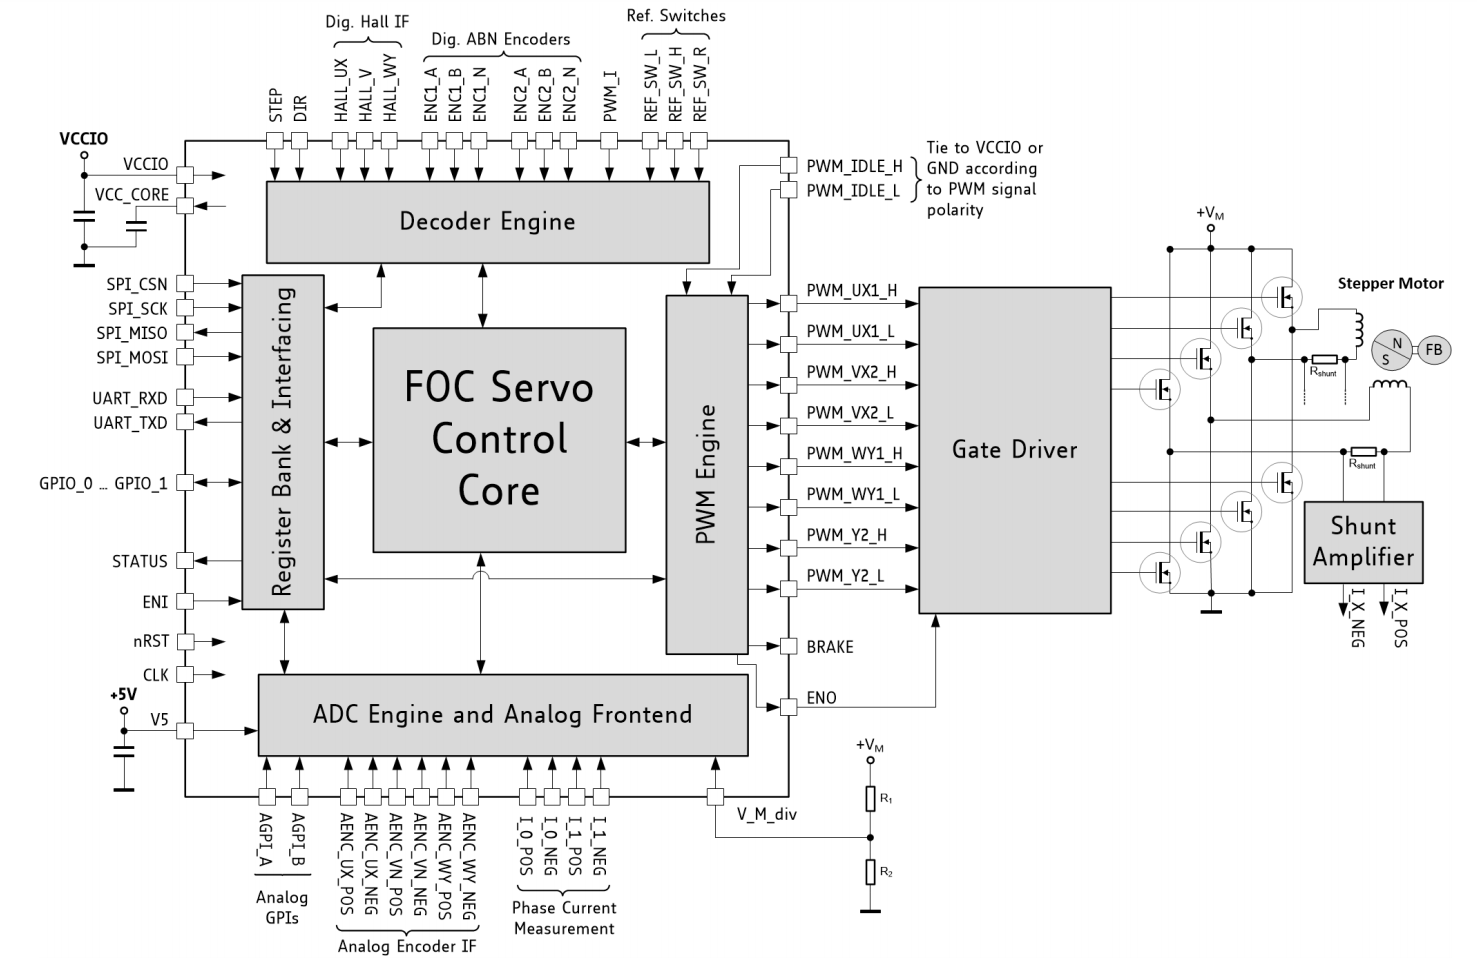
\includegraphics[width=0.8\textwidth]{graphics/Standard_Application_Cirquit_TMC4671}
	\caption{Standard-Anwendungs-Schaltung.}
	\label{fig:Schaltung_TMC4671}
\end{figure}
\todo{cite{TMC4671 Datenblatt}}

\subsection{Blockdiagramm TMC4671}

\begin{figure}[h!]
	\centering
	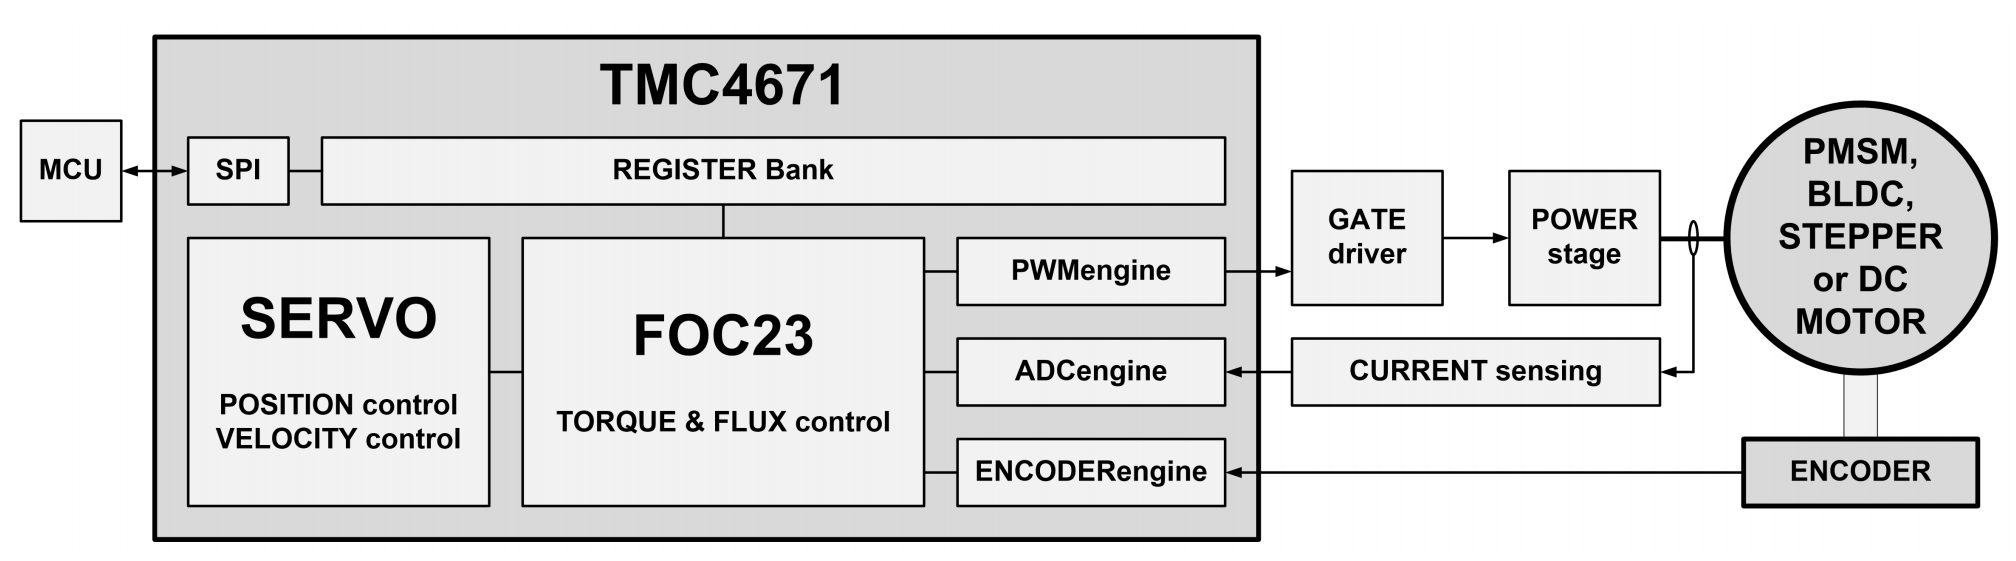
\includegraphics[width=0.8\textwidth]{graphics/Blockdiagramm_TMC4671}
	\caption{Blockdiagramm TMC4671.}
	\label{fig:Blockdiagramm_TMC4671}
\end{figure}

\todo{cite{TMC4671 Datenblatt}}

\newpage

\subsection{Inbetriebnahme Gate-Control}

\begin{figure}[h!]
\center
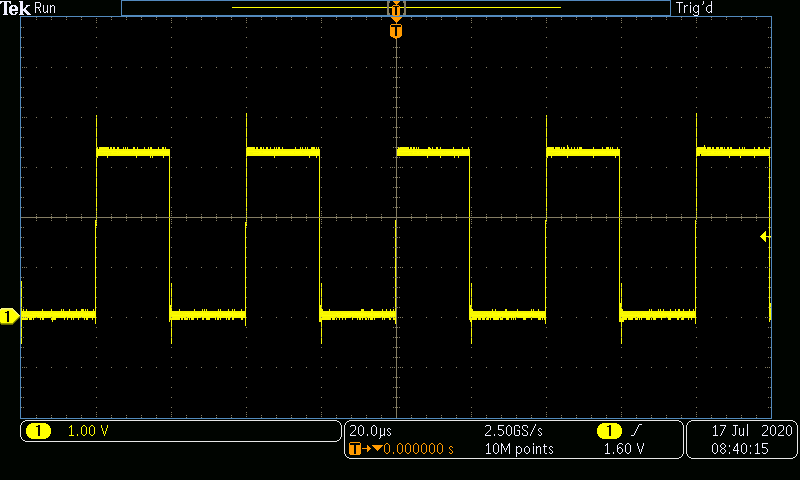
\includegraphics[width = 0.8\textwidth]{graphics/PWM_UX1_H}
\caption{Steuersignal PWM\_UX1\_H}
\label{fig:PWM_UX1_H}
\end{figure}

\begin{figure}[h!]
\center
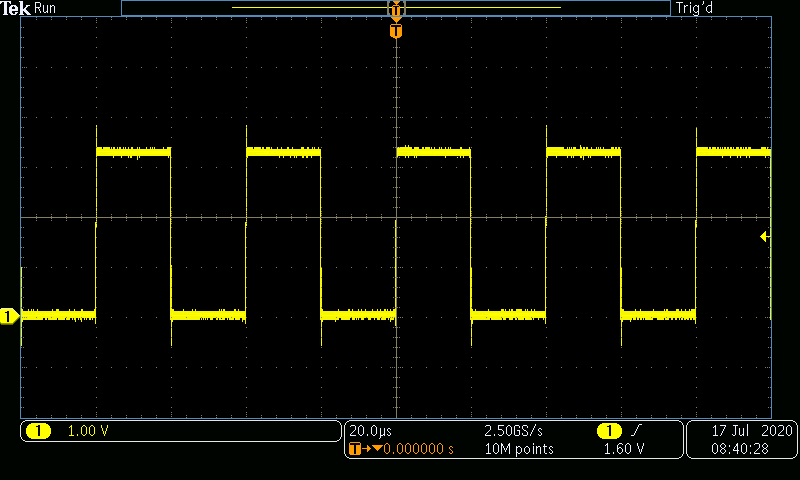
\includegraphics[width = 0.8\textwidth]{graphics/PWM_UX1_L}
\caption{Steuersignal PWM\_UX1\_L}
\label{fig:PWM_UX1_L}
\end{figure}

\newpage

\begin{figure}[h!]
\center
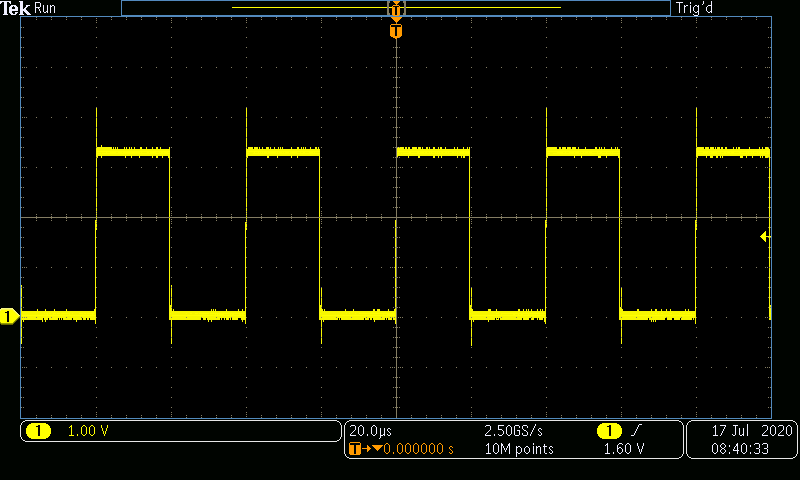
\includegraphics[width = 0.8\textwidth]{graphics/PWM_UX2_H}
\caption{Steuersignal PWM\_UX2\_H}
\label{fig:PWM_UX2_H}
\end{figure}

\begin{figure}[h!]
\center
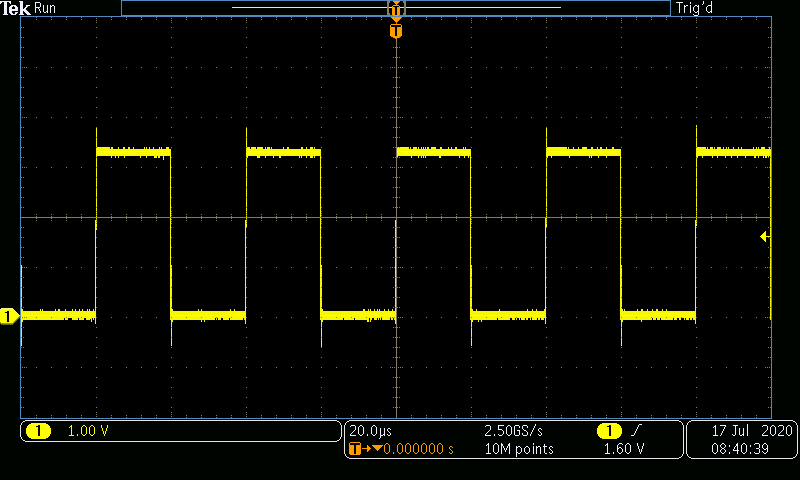
\includegraphics[width = 0.8\textwidth]{graphics/PWM_UX2_L}
\caption{Steuersignal PWM\_UX2\_L}
\label{fig:PWM_UX2_L}
\end{figure}

\newpage

\begin{figure}[h!]
\center
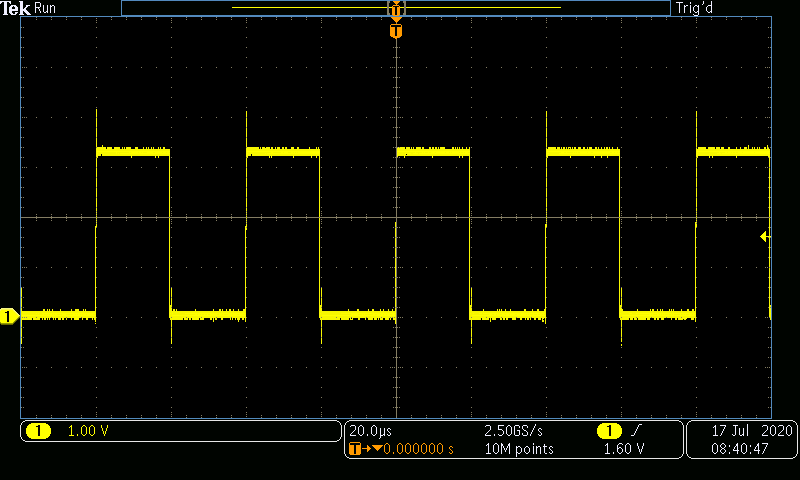
\includegraphics[width = 0.8\textwidth]{graphics/PWM_UX3_H}
\caption{Steuersignal PWM\_UX3\_H}
\label{fig:PWM_UX3_H}
\end{figure}

\begin{figure}[h!]
\center
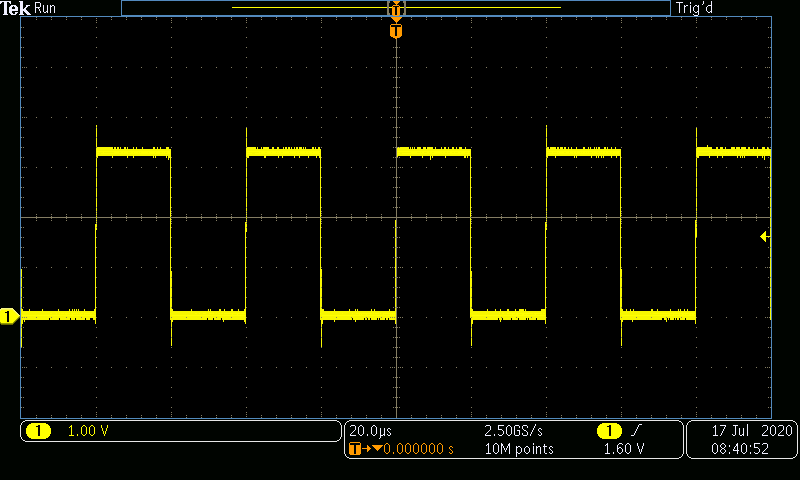
\includegraphics[width = 0.8\textwidth]{graphics/PWM_UX3_L}
\caption{Steuersignal PWM\_UX3\_L}
\label{fig:PWM_UX3_L}
\end{figure}

\newpage


\begin{figure}[h!]
\center
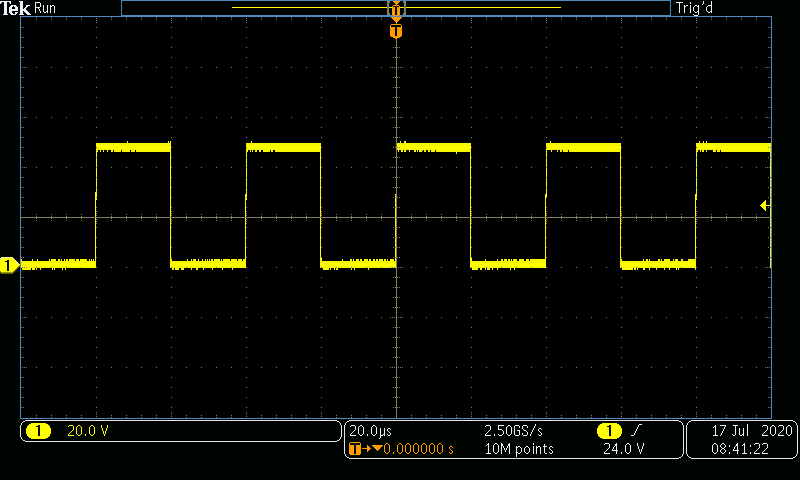
\includegraphics[width = 0.8\textwidth]{graphics/Motor_U}
\caption{Motorsignal U nach H-Brücke}
\label{fig:PWM_UX1_H}
\end{figure}

\begin{figure}[h!]
\center
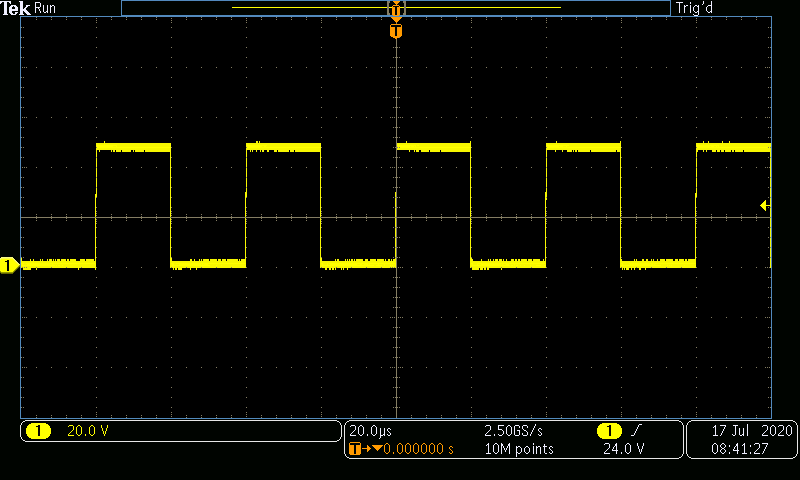
\includegraphics[width = 0.8\textwidth]{graphics/Motor_V}
\caption{Motorsignal U nach H-Brücke}
\label{fig:PWM_UX1_H}
\end{figure}

\newpage


\begin{figure}[h!]
\center
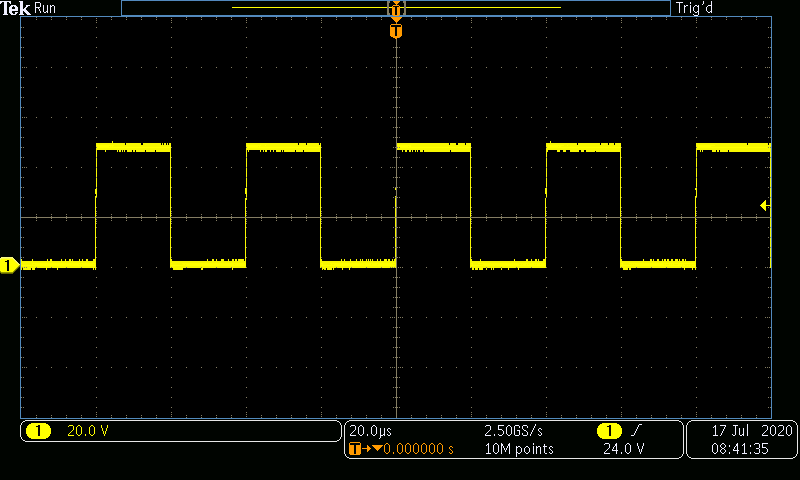
\includegraphics[width = 0.8\textwidth]{graphics/Motor_W}
\caption{Motorsignal U nach H-Brücke}
\label{fig:PWM_UX1_H}
\end{figure}


\newpage

\section{TMC6200}\label{Appendix:TMC6200}

\subsection{Standard-Schaltkreis TMC6200}

\begin{figure}[h!]
	\centering
	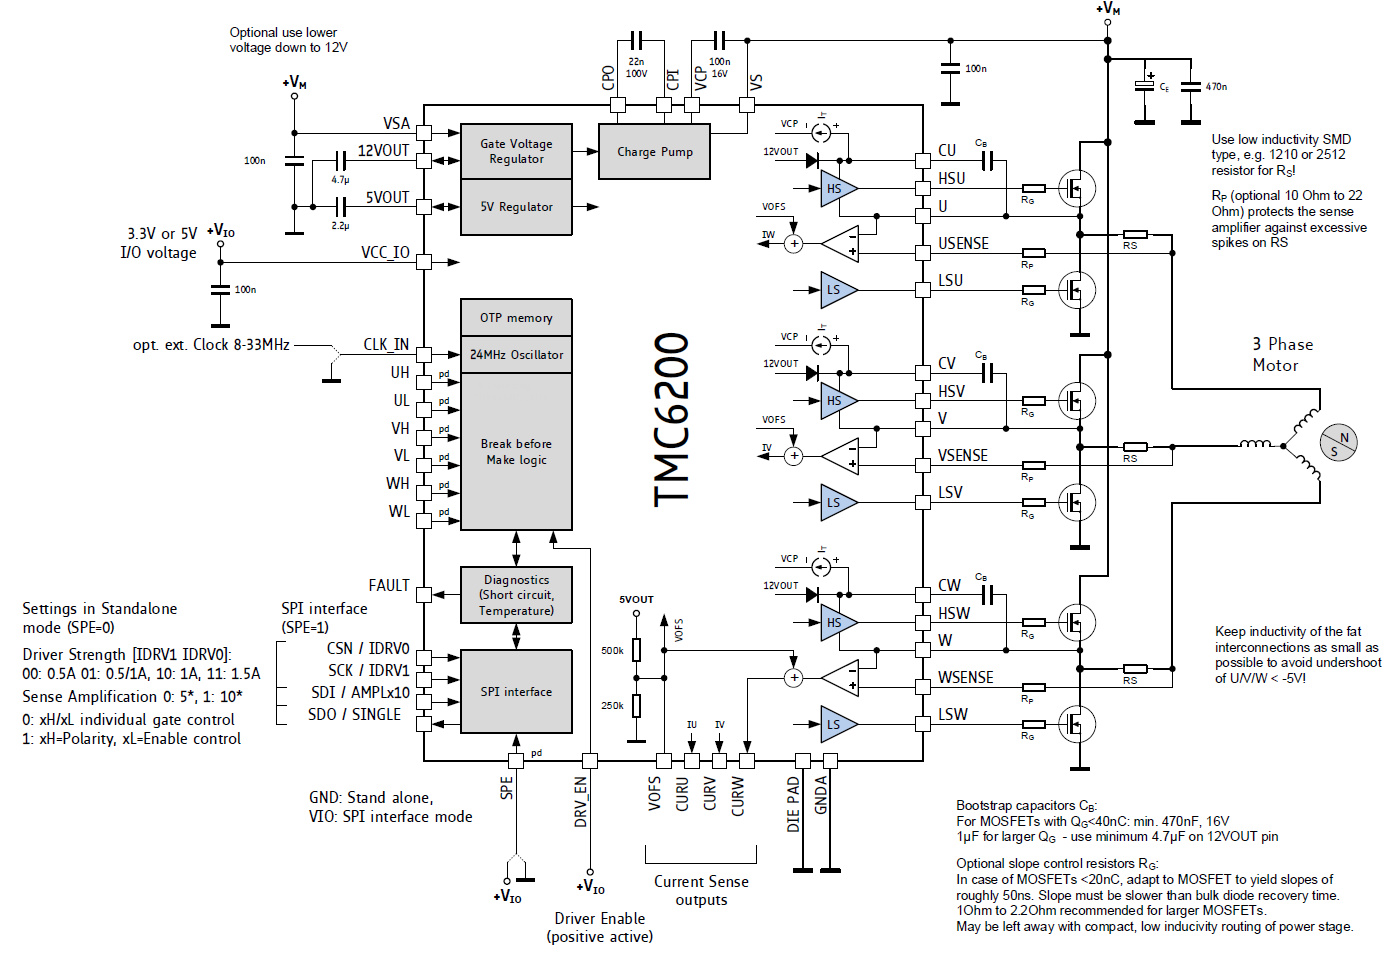
\includegraphics[width=0.8\textwidth]{graphics/Standard_Application_Cirquit_TMC6200.png}
	\caption{Standard-Anwendungs-Schaltung TMC6200.}
	\label{fig:Schaltung_TMC6200}
\end{figure}

\subsection{Blockdiagramm TMC6200}

\begin{figure}[h!]
	\centering
	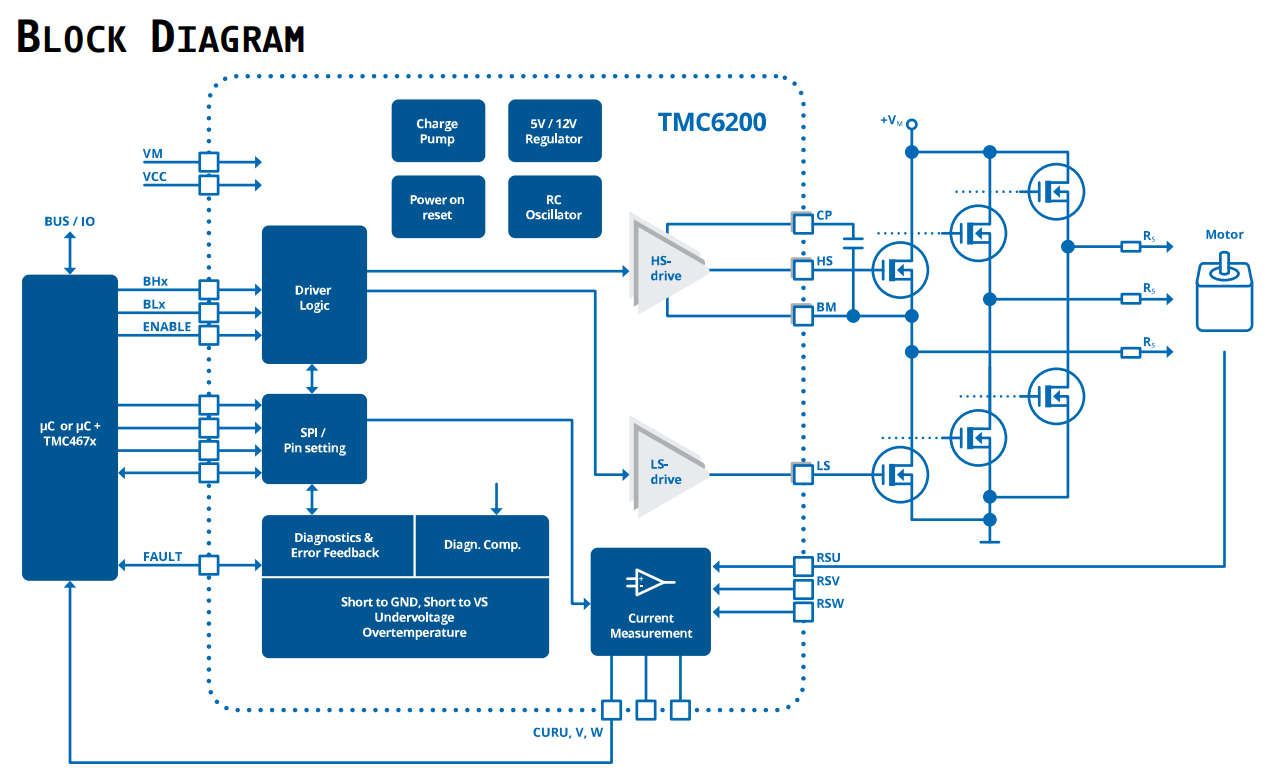
\includegraphics[width=0.8\textwidth]{graphics/Blockdiagramm_TMC6200.png}
	\caption{Blockdiagramm TMC6200.}
	\label{fig:Blockdiagramm_TMC6200}
\end{figure}

\newpage

\subsection{Verstärkungsfaktor, Strommessung, Strommesswiderstand}

\begin{figure}[h!]
	\centering
	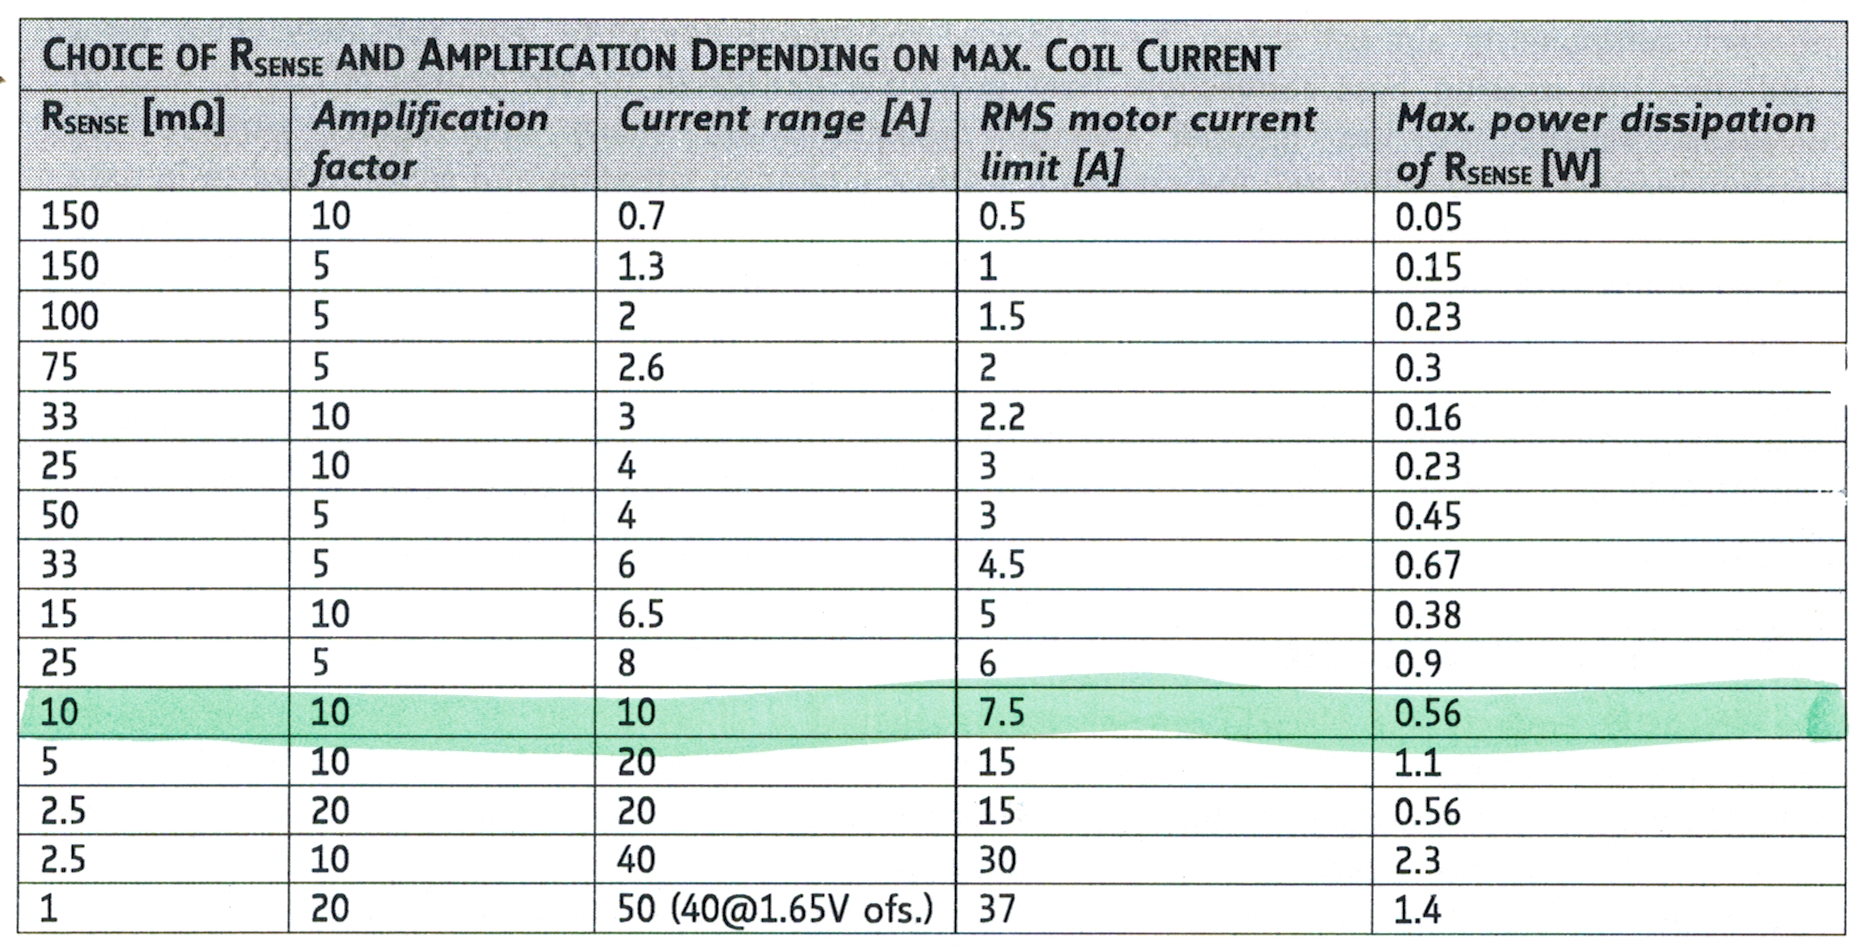
\includegraphics[width=\textwidth]{graphics/Tabelle_Shunts.png}
	\caption{Tabelle zur Bestimmung des Strommesswiderstandes aus dem Datenblatt von Trinamic.}
	\label{fig:Tabelle_Shunts}
\end{figure}

\subsection{Gate-Vorwiderstand}

\begin{figure}[h!]
	\centering
	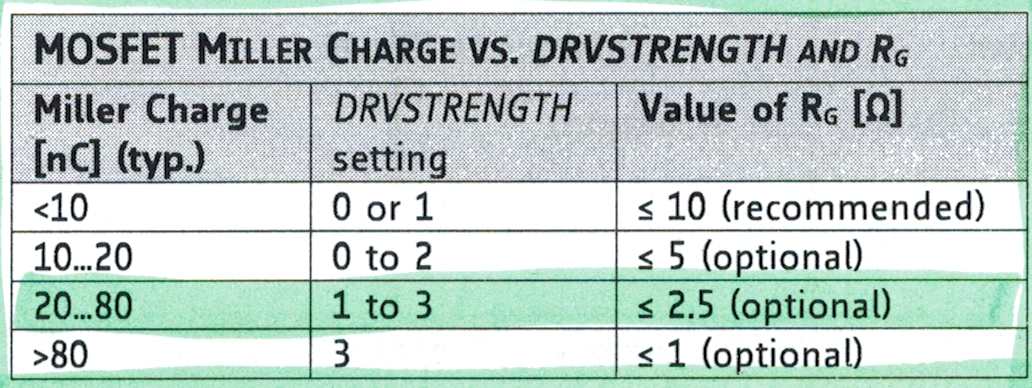
\includegraphics[width=0.5\textwidth]{graphics/Tabelle_Gatewiderstaende.png}
	\caption{Tabelle zur Bestimmung der Gatewiderstände aus dem Datenblatt von Trinamic.}
	\label{fig:Tabelle_Gatewiderstaende}
\end{figure}

\subsection{Externe Gate-Spannungsversorgung}

\begin{figure}[h!]
	\centering
	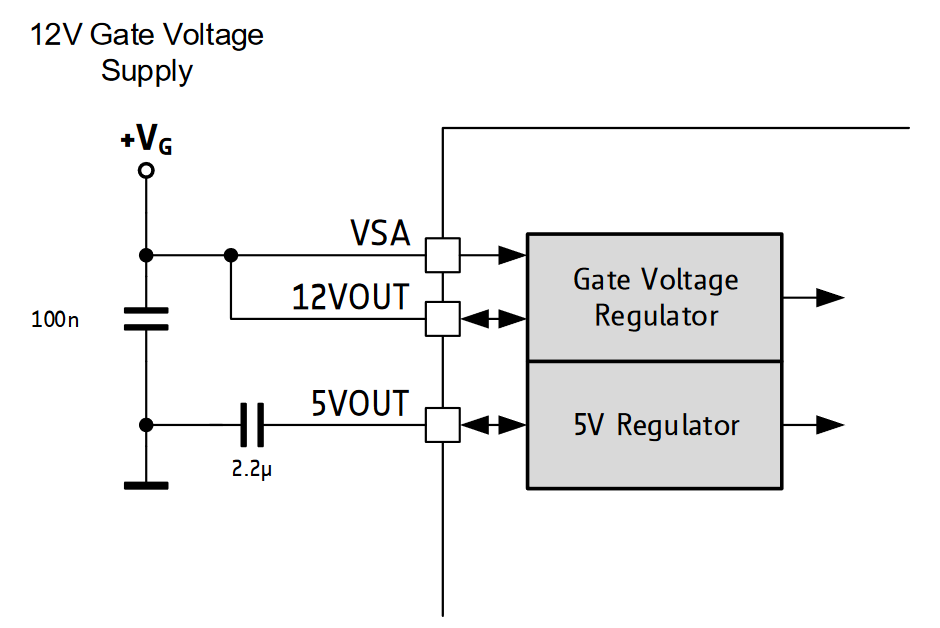
\includegraphics[width=0.5\textwidth]{graphics/Schema_Gate_Treiber_Gatespannung}
	\caption{Schema externe Gate-Spannungsversorgung.}
	\label{fig:Schema_Gate_Treiber_Gatespannung}
\end{figure}

\newpage

\section{H-Brücke}\label{Appendix:H_Bruecke}

\subsection{Referenzschema}

\begin{figure}[h!]
	\centering
	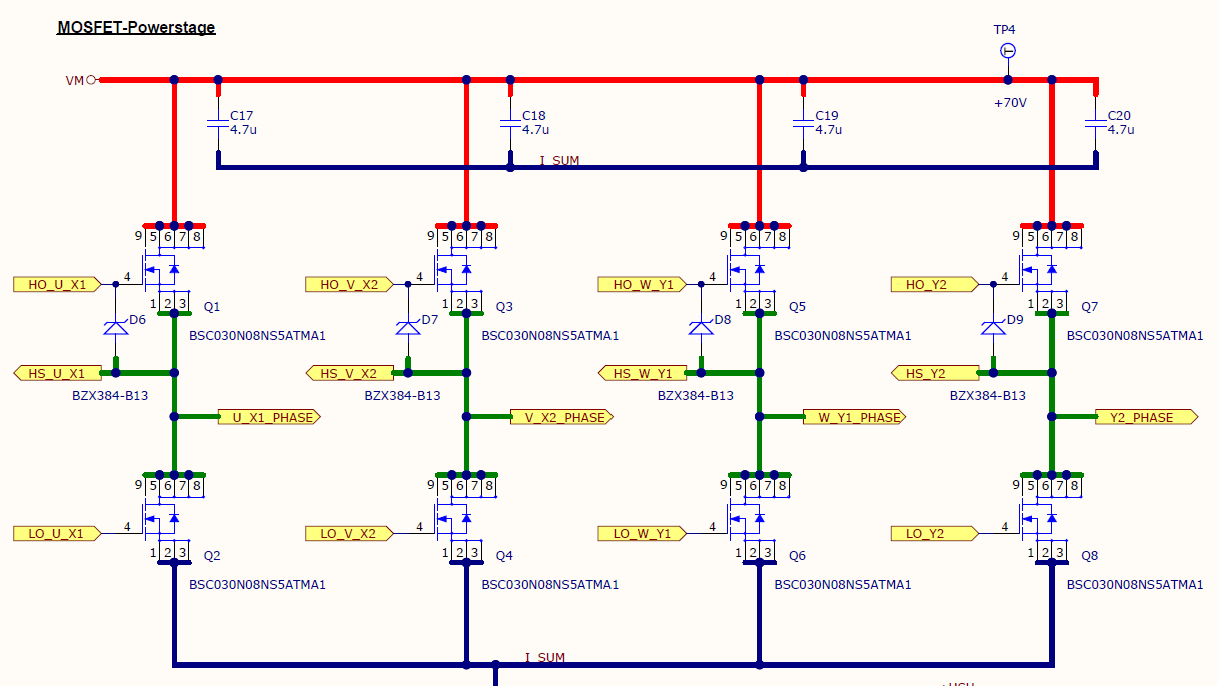
\includegraphics[width=0.7\textwidth]{graphics/Referenzschema_10A70V}
	\caption{H-Brücke.}
	\label{fig:Schema_H_Bruecke_und_BLDC_Ref}
\end{figure}

\todo{cite: Datenblatt UPS 10A70V Schema}

\section{Mikrocontroller}\label{Appendix:Mikrocontroller}

\subsection{Brown-out-Detection}\label{Appendix:Brown-out-Detection}

\begin{figure}[h!]
	\centering
	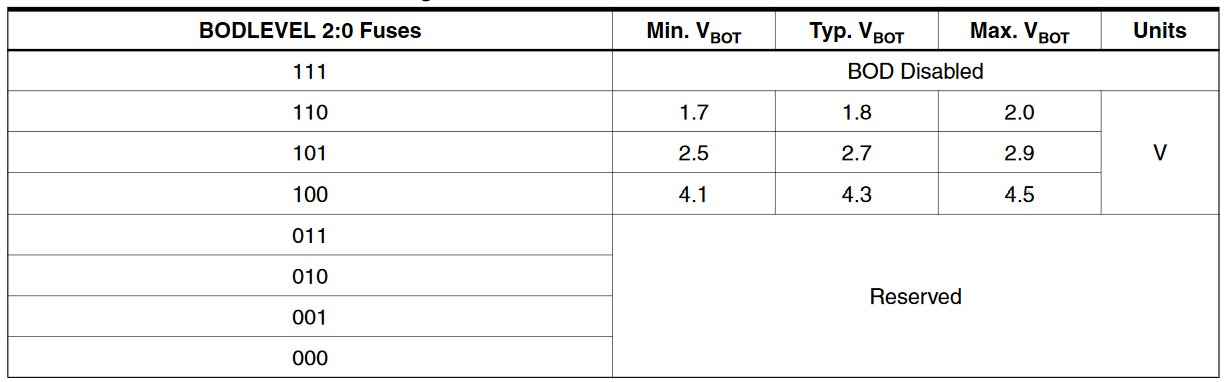
\includegraphics[width=0.7\textwidth]{graphics/Tabelle_BoD}
	\caption{Tabelle Brown-out-Detection.}
	\label{fig:Tabelle_BoD}
\end{figure}

\todo{cite: Datenblatt Atmega 2560, Seite 361}

\subsection{Full Swing Crystal Oscillator}\label{Appendix:Full_Swing _Crystal_Oscillator}

\begin{figure}[h!]
	\centering
	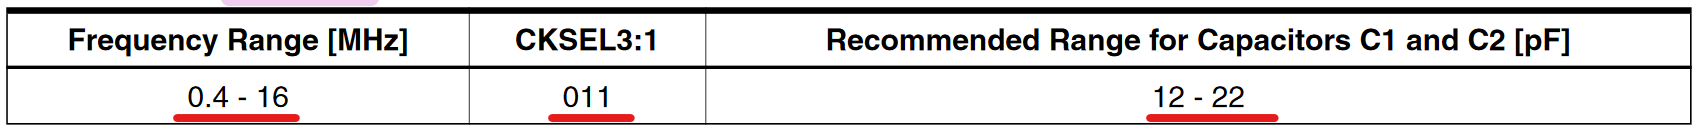
\includegraphics[width=0.7\textwidth]{graphics/Tabelle_Crystal}
	\caption{Tabelle Frequenzbereich Crystal Oszillator.}
	\label{fig:Tabelle_Crystal}
\end{figure}

\todo{cite: Datenblatt Atmega 2560, Seite 43}

\newpage

\begin{figure}[h!]
	\centering
	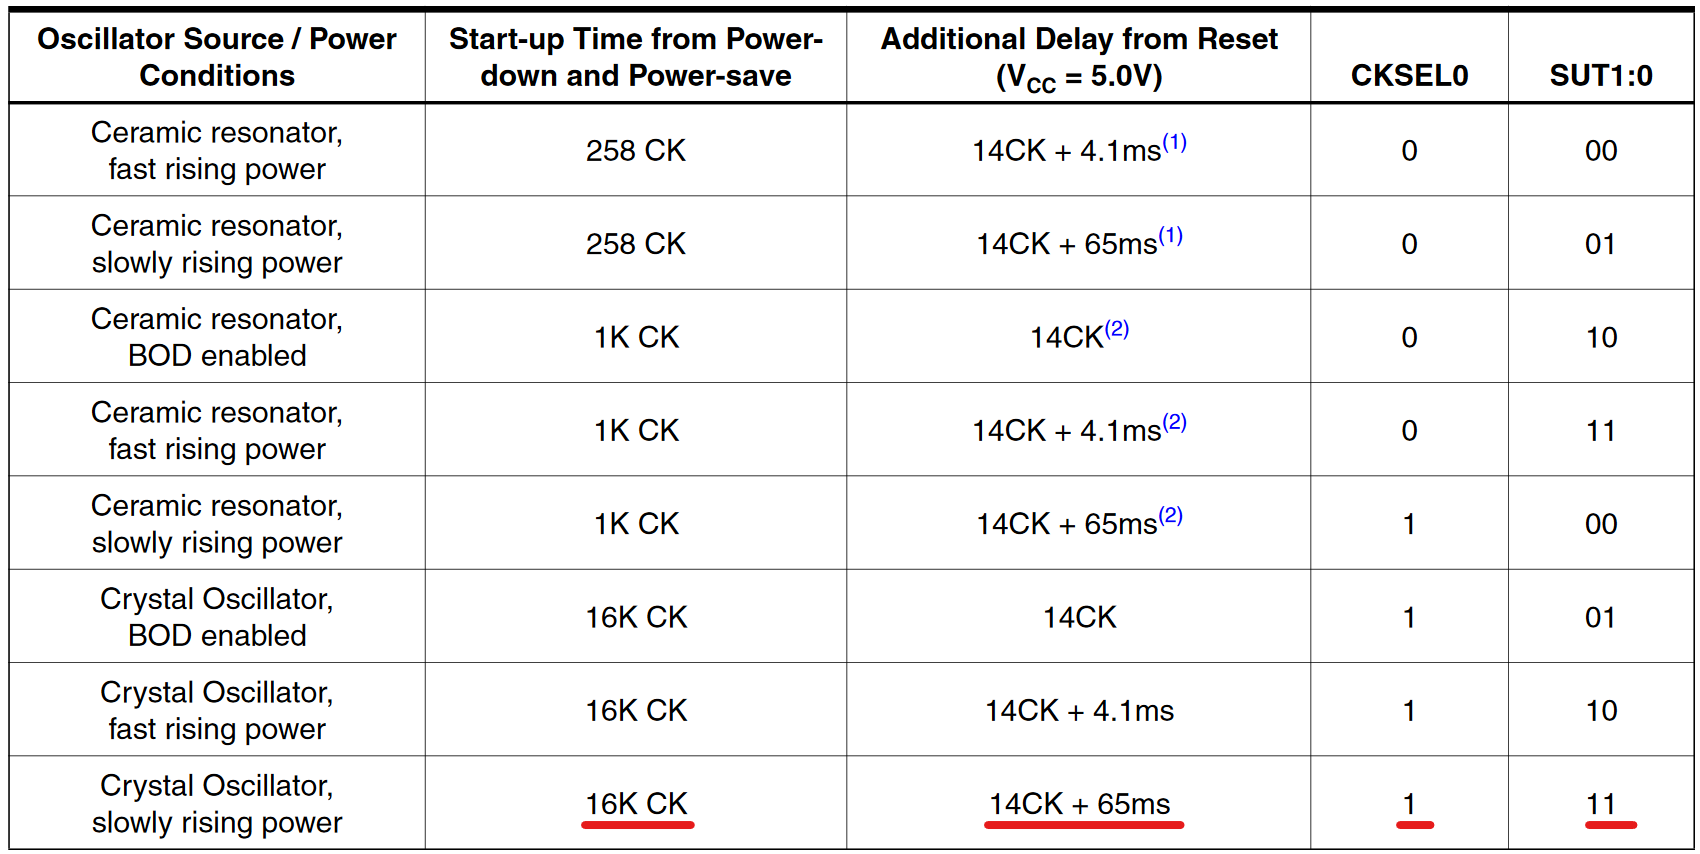
\includegraphics[width=0.7\textwidth]{graphics/Tabelle_Crystal2}
	\caption{Tabelle Aufstartzeit.}
	\label{fig:Tabelle_Crystal2}
\end{figure}

\todo{cite: Datenblatt Atmega 2560, Seite 43}

\subsection{Bootloader-Speicherplatz}\label{Appendix:Bootloader-Speicherplatz}

\begin{figure}[h!]
	\centering
	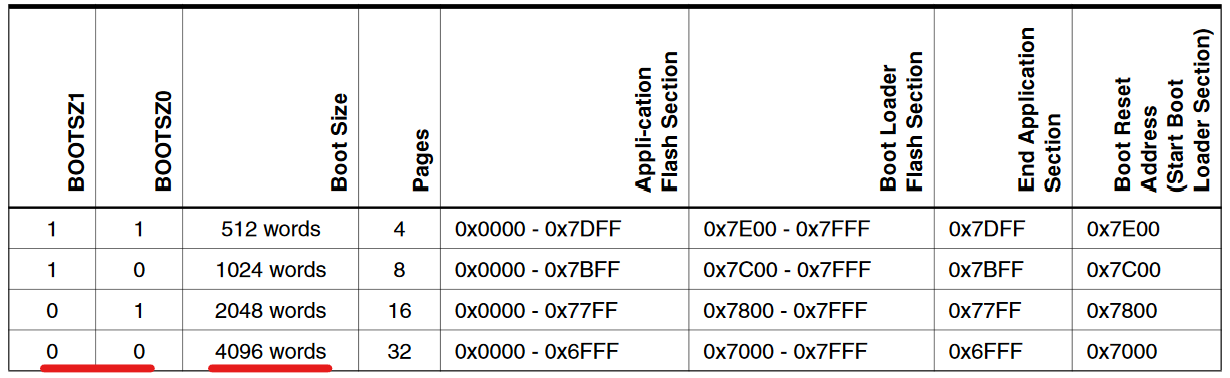
\includegraphics[width=0.7\textwidth]{graphics/Tabelle_Bootloader}
	\caption{Tabelle Bootloader Speicherplatz.}
	\label{fig:Tabelle_Bootloader}
\end{figure}

\todo{cite: Datenblatt Atmega 2560, Seite 320}

\subsection{Memory-Lock Bootloader}

\begin{figure}[h!]
	\centering
	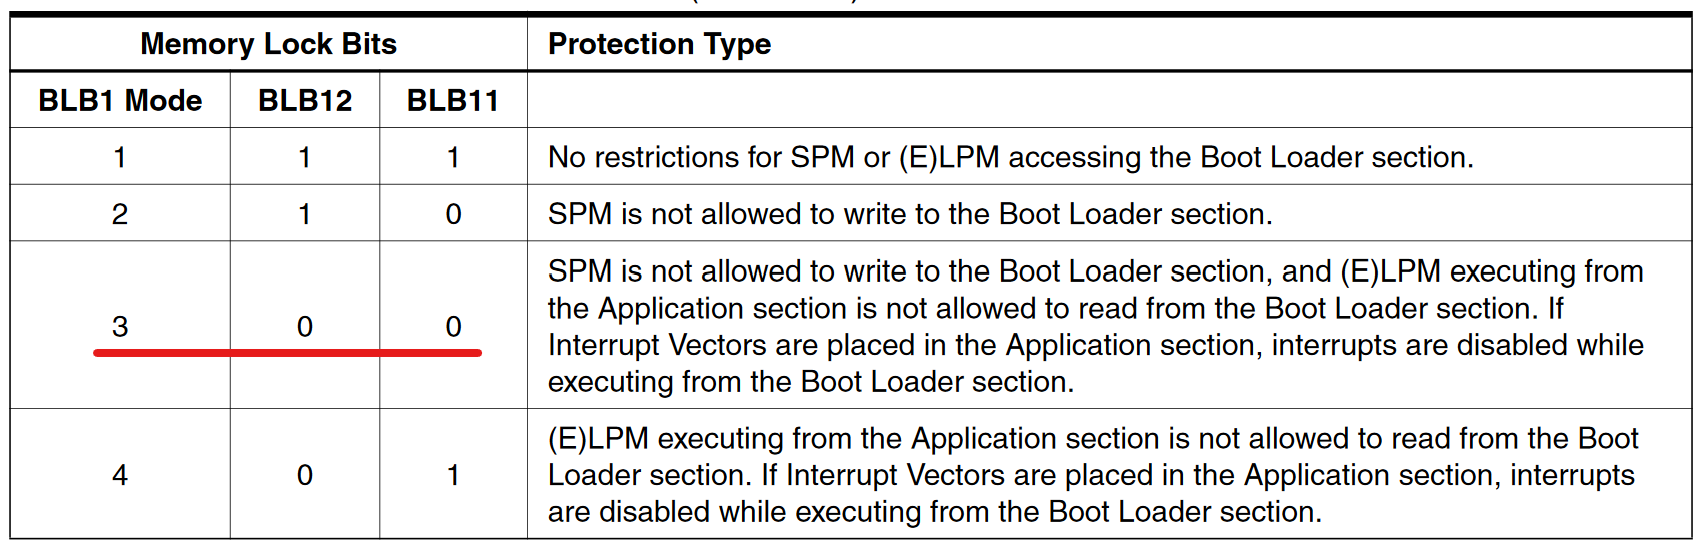
\includegraphics[width=0.7\textwidth]{graphics/Tabelle_Memory_Lock}
	\caption{Tabelle Memory Lock.}
	\label{fig:Tabelle_Memory_Lock}
\end{figure}

\todo{cite: Datenblatt Atmega 2560, Seite 326}

\newpage
\section{USB-B}\label{Appendix:USB_B}

\subsection{Geräte-Manager}

\begin{figure}[h!]
\center
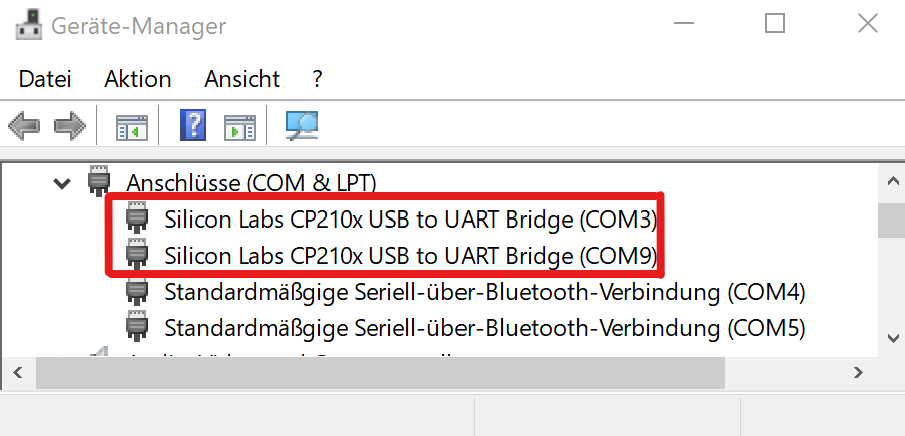
\includegraphics[width = 0.6 \textwidth]{graphics/USB_Devices_Ger_Man}
\caption{Geräte-Manager mit den aufgelisteten USB-UART-Converter (Mikrocontroller und WiFi-Modul).}
\label{fig:USB_Devices_Ger_Man}
\end{figure}

\section{Atmel Studio}\label{Appendix:Atmel_Studio}

\subsection{Fuse Bits}

\begin{figure}[h!]
	\centering
	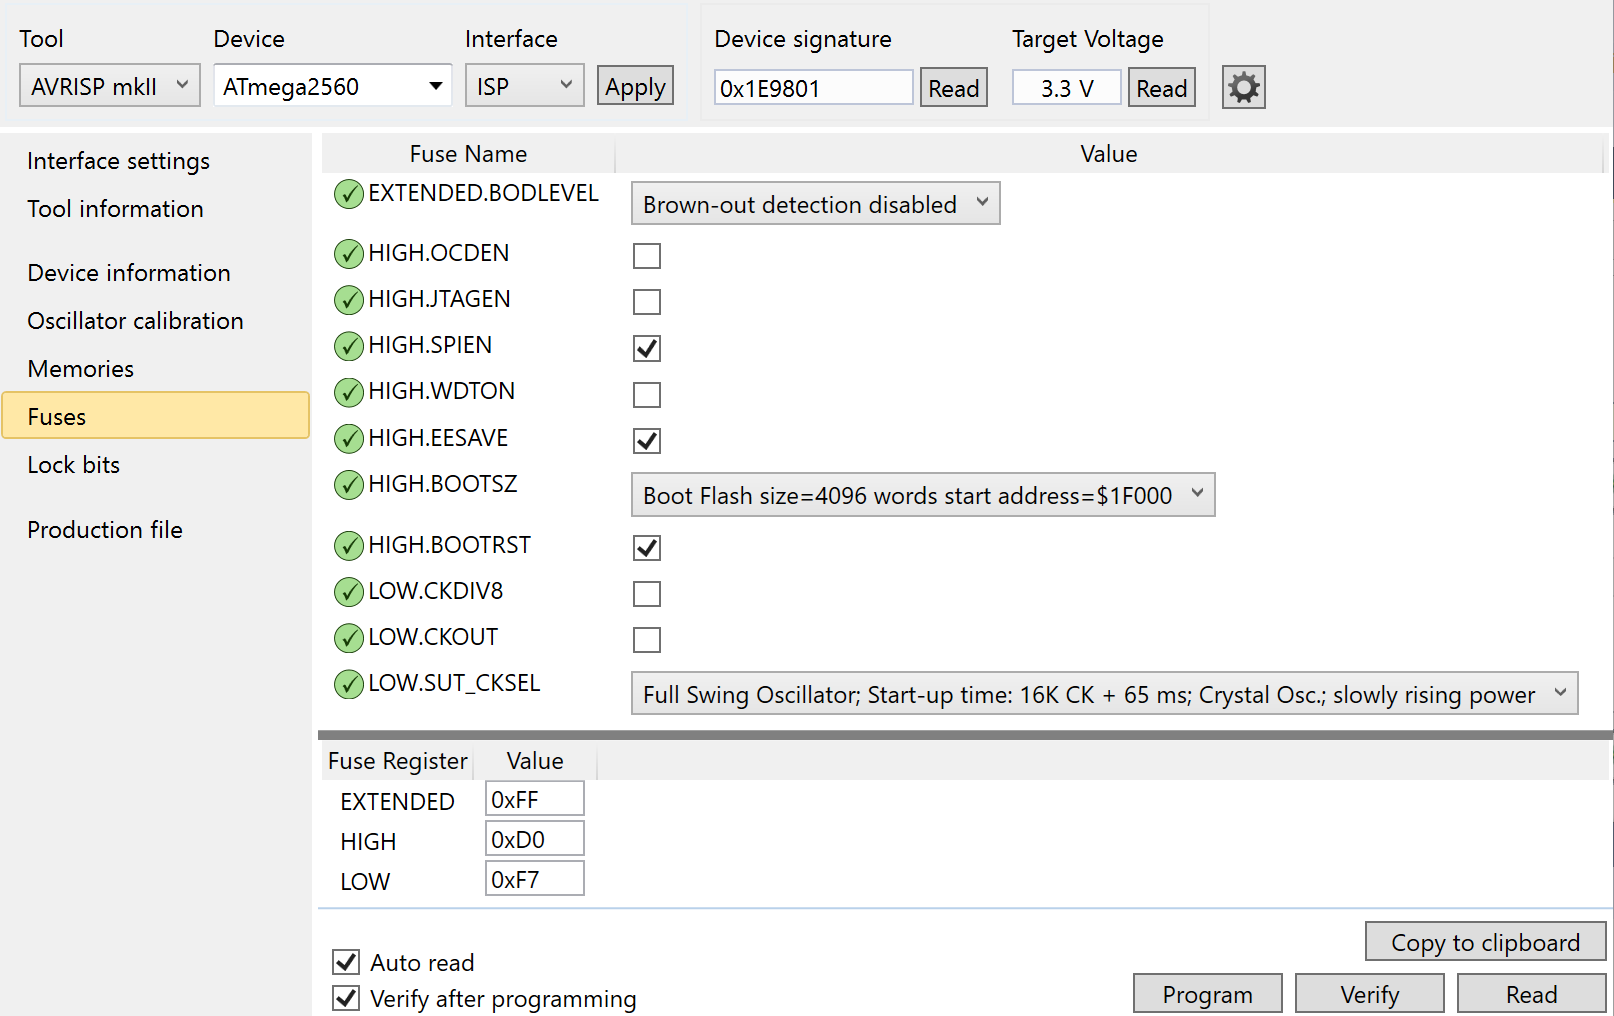
\includegraphics[width=\textwidth]{graphics/AtmelStudio_Fuses}
	\caption{Fuse-Bits Atmega2560.}
	\label{fig:AtmelStudio_Fuses}
\end{figure}

\subsection{Lock Bits}

\begin{figure}[h!]
	\centering
	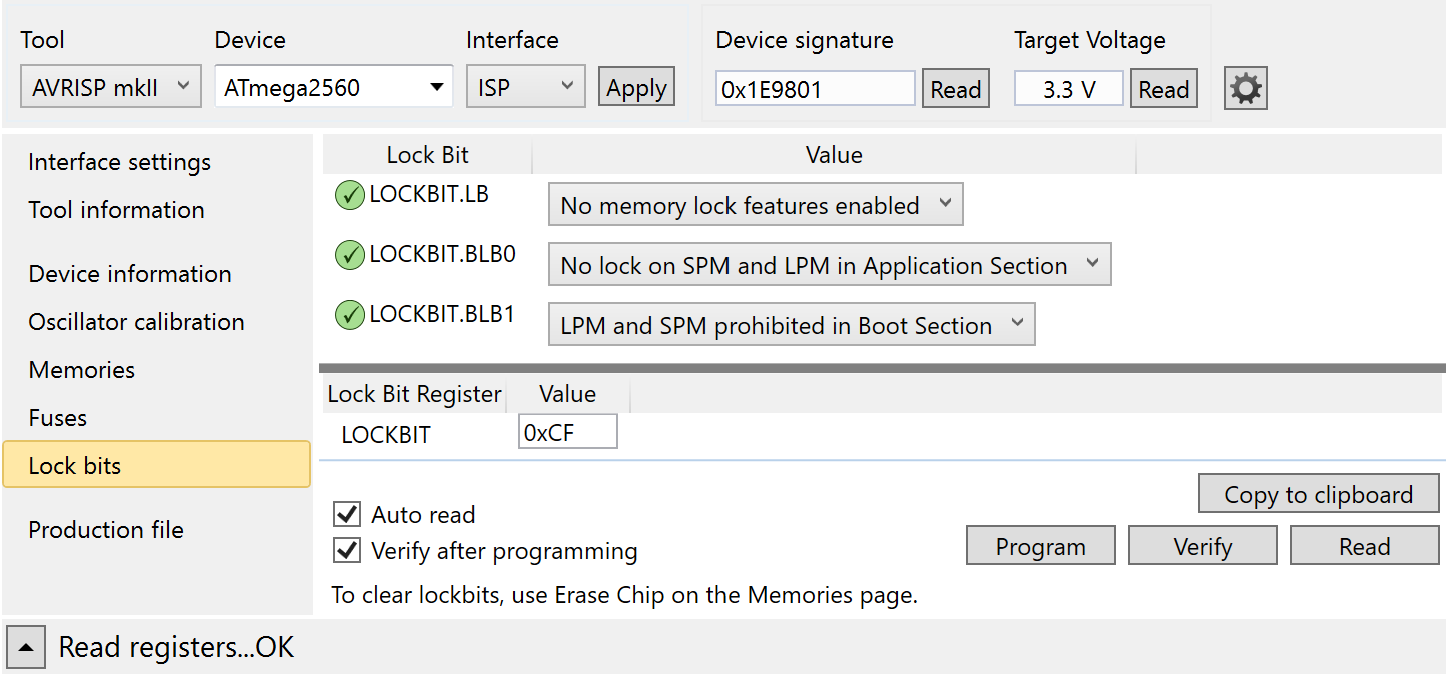
\includegraphics[width=\textwidth]{graphics/AtmelStudio_Locks}
	\caption{Lock-Bits Atmega2560.}
	\label{fig:AtmelStudio_Locks}
\end{figure}
\newpage
\subsection{Einbinden AVRdude und stk500v2 (wiring)}

\begin{figure}[h!]
	\centering
	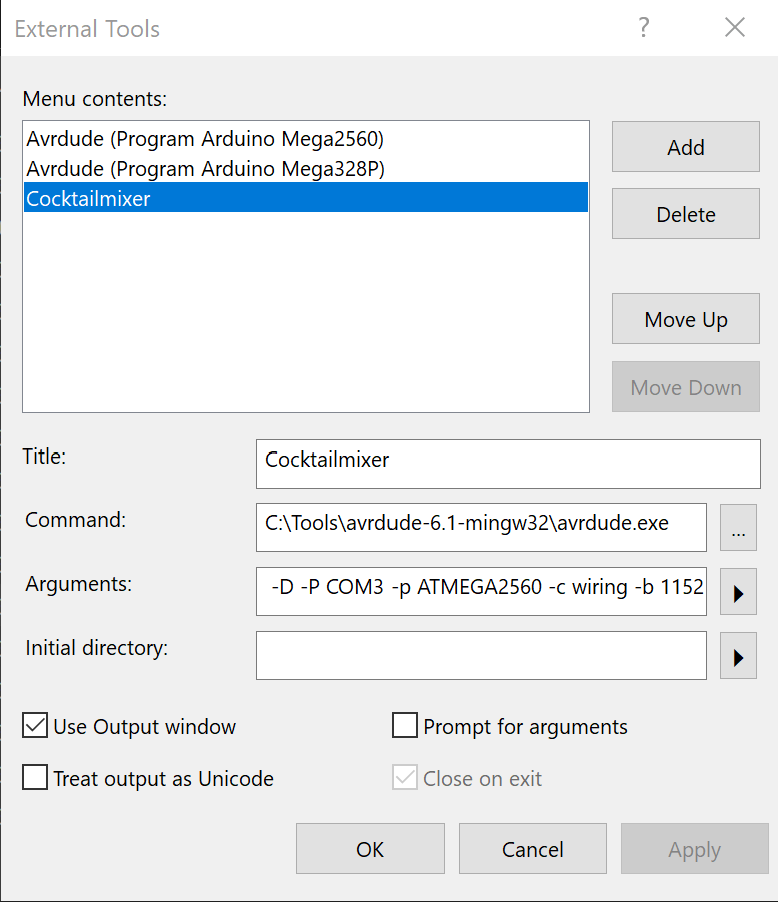
\includegraphics[width=0.5\textwidth]{graphics/AtmelStudio_External_Tools}
	\caption{External Tools Atmega2560.}
	\label{fig:AtmelStudio_Locks}
\end{figure}

\subsection{Bootloader ''Brennen''}

\begin{figure}[h!]
	\centering
	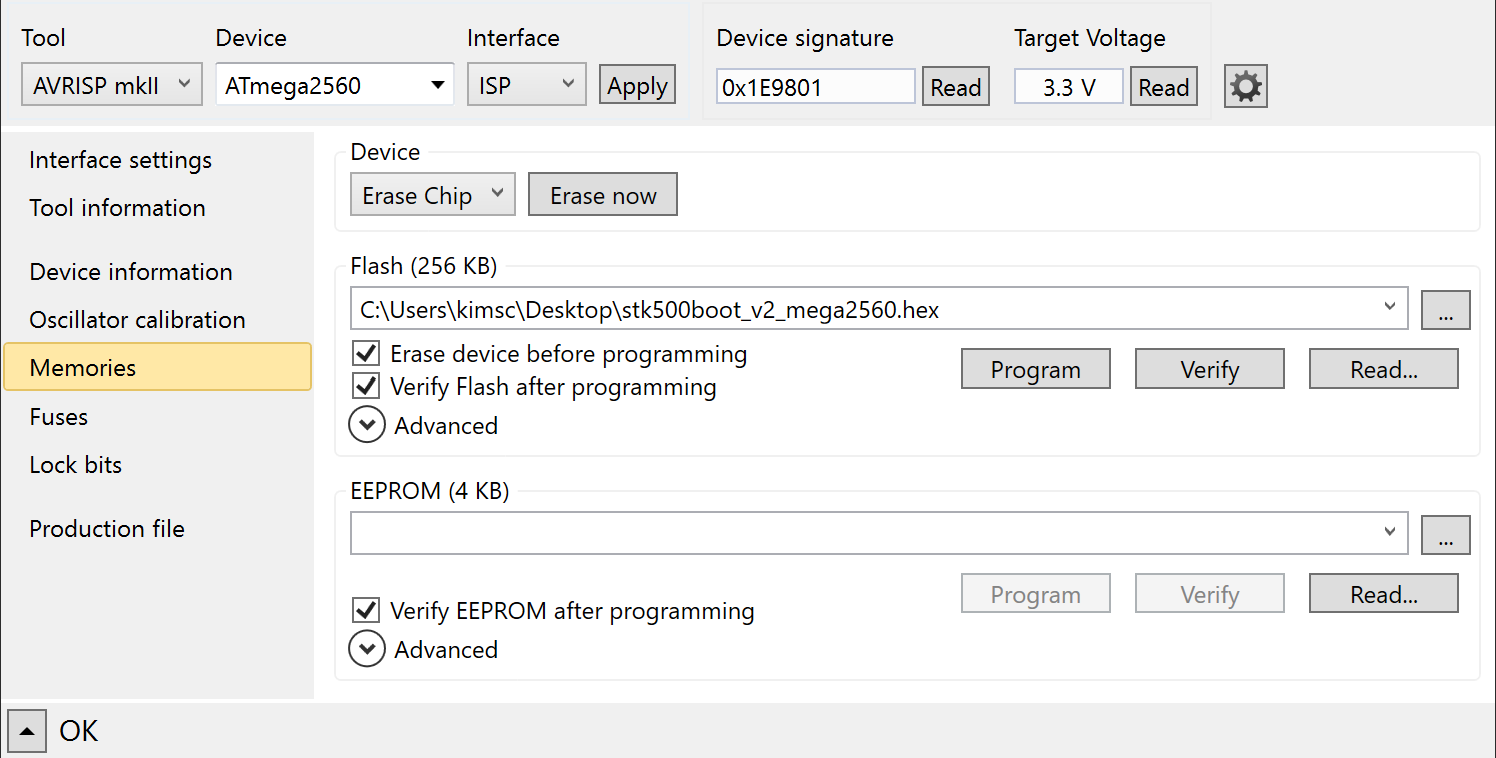
\includegraphics[width=\textwidth]{graphics/AtmelStudio_Program_Bootloader}
	\caption{Bootloader brennen.}
	\label{fig:AtmelStudio_Program_Bootloader}
\end{figure}

\end{appendix}

%%---NOTES for DEBUG---------------------------------------------------------------------
\ifdraft{%Do this only if mode=draft
%%requires \usepackage{todonotes})
\newpage
\listoftodos[\section{Todo-Notes}]
\clearpage
}
{%Do this only if mode=final
}

\end{document}
